\documentclass[rnd]{mas_proposal}
% \documentclass[thesis]{mas_proposal}

\usepackage[utf8]{inputenc}
\usepackage{amsmath}
\usepackage{amsfonts}
\usepackage{amssymb}
\usepackage{graphicx}
\usepackage{lscape} % For table landscape view
% \usepackage[nottoc]{tocbibind} % To add list of tables and figures to toc
% \usepackage[style=super4col, acronym]{glossaries}
\usepackage{float}
\usepackage{multirow}

\title{Navigation of Bulky Robots in Confined Indoor Spaces}
\author{Devaiah Ulliyada Arun}
\supervisors{Prof. Dr. Erwin Prassler\\
Prof. Nico Hochgeschwender\\
Dipl.-Ing. Nico Hübel
}
\date{May 2022}

% \thirdpartylogo{path/to/your/image}

\begin{document}

\maketitle

\pagestyle{plain}

\section{Introduction}
Navigation in indoor structured environment includes traversing in different settings such as open spaces, narrow confined static spaces or heavily crowded dynamic areas as shown in Figure \ref{Fig:indoor-map}. Areas where the robot can use all the degrees of freedom of motion securely, are considered open spaces. The rest of the spaces are restricted or forbidden based on the size of the robot. Global planning requires accessibility of environmental and robot odometric information to obtain an accurate and optimal path. The shortest path is considered as the time saving constraint and the safest path is considered as the safety constraints for mobile robots. To satisfy such requirement, there are many path planning methods already proposed by researchers.

\begin{figure}[!ht]
\centering
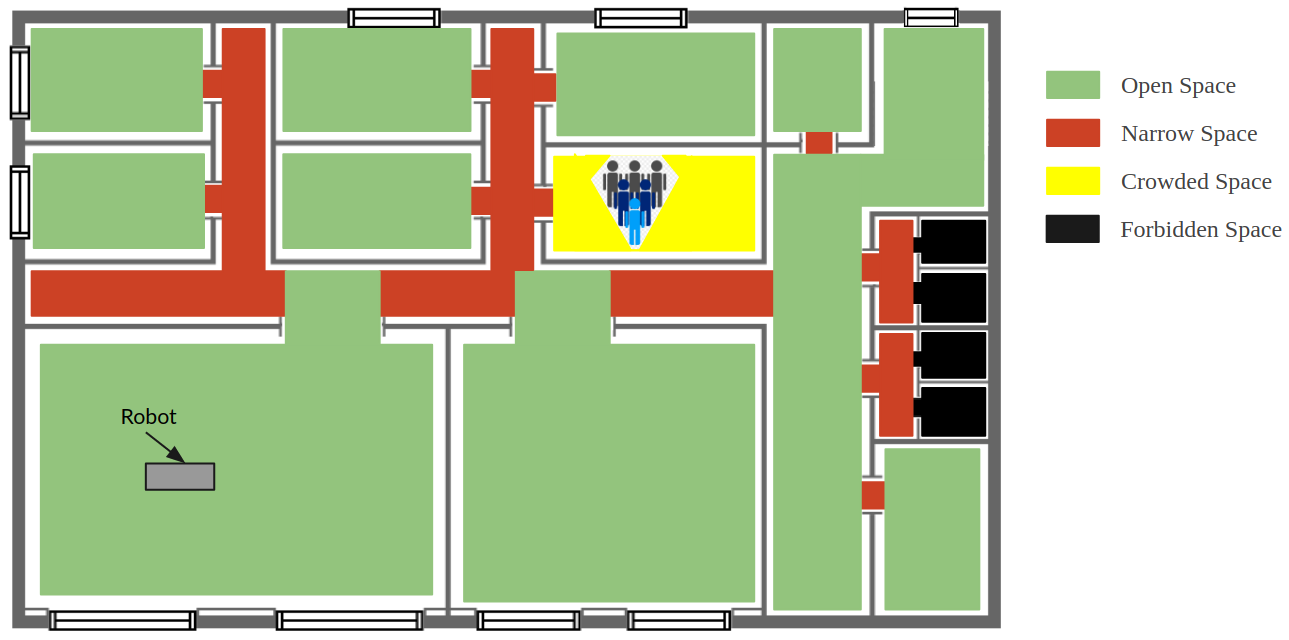
\includegraphics[scale=0.3]{images/Indoor_Map.png}
\caption{Indoor structured environment with areas with different spaces.}
\label{Fig:indoor-map}
\end{figure}

Traditional planners, usually built for long range navigation tend to inefficiently solve navigation in confined spaces or could fail to solve it. However, one can find few useful solutions for scenarios where the robot has to cross narrow or cluttered areas. The solutions available are either specific to certain scenarios or particular robot platforms or mainly handle forward motion control. Another level of complexity would be added if the robot has constraints. Irregular polygon shape (edges are unequal) of the robot allows it to exist only in certain poses in confined space. Considering bulky logistic robots as shown in Figure \ref{Fig:robot-platform}, the length of the robot is larger than most width of narrow corridors.

\begin{figure}[!ht]
\centering
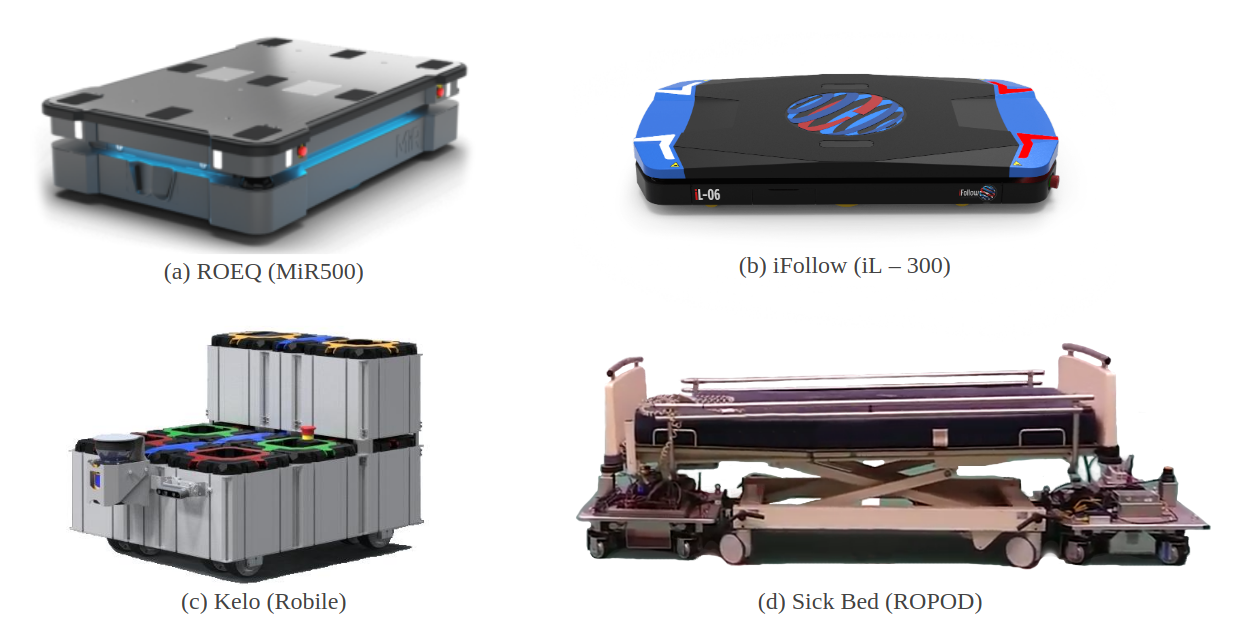
\includegraphics[scale=0.33]{images/Robot Platform.png}
\caption{Non square bulky robotic platform (a) 1304 x 864 x 95 (mm) (b) 1435 x 760 x 176 (mm) (c) 690 x 460 x 230 (mm).}
\label{Fig:robot-platform}
\end{figure}

Use cases for confined space planning includes traversing through corridors, intersections, doorways and dynamic obstacles restricting open spaces. For bulky robots, navigating through such environments poses a safety concern. Maneuvering through it requires the robot to use forward and reverse curved motions as shown in Figure \ref{Fig:use-case}. 

\begin{figure}[!ht]
\centering
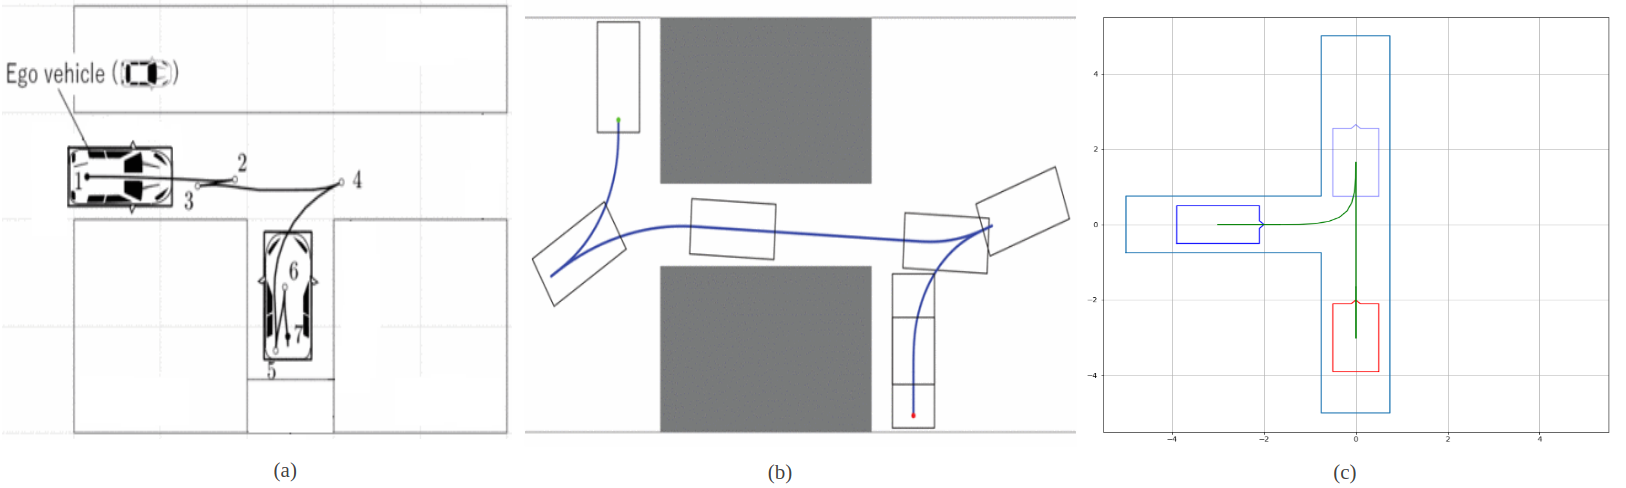
\includegraphics[width=14.5cm,height=6cm]{images/Use cases.png}
\caption{(a) Reverse parking (b) Maneuvering in narrow corridor (c) Maneuvering through intersection.}
\label{Fig:use-case}
\end{figure}

\section{Related Work}
The related work is categorized to physics based, robot planning and automotive planning approaches based on its applications.
\subsection{Physics Based Approaches}
Earlier works on narrow space planning were classically formulated as the ‘Piano Mover's Problem’. These approaches assumes a single object moving in a static, completely known environment without any dynamic constraint. It guarantees to find a path if one exists at a given environment resolution and all the paths that it returns are safe.
Although a path is guaranteed, the complexity grows exponentially with the number of degrees of freedom of the robot. Also, the approaches become highly inefficient in dynamic environments. 

Near optimal planning approaches proposed by \cite{1225154} and \cite{1511035} considers a rectangular object traversing through narrow spaces. The approach decomposes the environment into square cells, each carrying a set of information which forms the cost function. The motion primitives uses the 8-geometry maze router including discretized rotation. Finally, a shortest and safest path is obtained using backtracking with minimum cost. The main drawback of such an approach is that the complexity increases as the resolution or size of the environment or number of motion primitives increase and hence is not suitable for long range navigation. 

Another way to formulate the piano mover's problem is proposed by \cite{6821131}, where the problem considers a moving ladder in configuration space. The valid regions are expressed logically by including quantifiers and then Quantifier Elimination by Partial CAD (QEPCAD) is used to construct cells describing a set of semi-algebraic equations expressing the validity of the cell for a particular configuration of the ladder. Finding adjacency and connectedness of cells in the four-dimensional CAD is not currently possible with any existing technology. This is just a new way to formulate the problem and maybe could produce a solution in the future.

\subsection{Robot Planning Approaches}
General robot planning in indoor environment, first renders the environment to accommodate the planner by using cell decomposition or applying potential field or setting heuristic rules. Roadmap approaches such as Voronoi diagram, visibility graph, and some other topological retractions are also popular. Most papers use some robot dimensional information to represent the environment creating a configuration space for narrow space planning. Finally, path planning uses potential field algorithm, sampling based algorithm or heuristic search algorithm along with optimization to find a smooth collision path. To tackle dynamic environment, local planners such as Dynamic Window Approach or Elastic Bands can also be implemented.

A* planning approaches \cite{6876211} \cite{6968200} can be modified to be applied to configuration space where each step includes checking the collision with the edges of the robot. This way of searching becomes very inefficient in long range planning. A* can also be used to obtain an initial coarse path which can later be optimized based on the robot and environment constraints \cite{9632369} \cite{8743249} \cite{8484297}. The drawback with this approach is that the robot can get stuck in local minima if the initial reference path is not in the direction of the optimal path.

Sampling based search like Rapid Random Trees (RRTs) explore large environments quicker compared to search based algorithms. But they are slow while exploring narrow spaces. There are many extensions to RRTs to efficiently explore confined spaces. Sampling using bridge test \cite{8961757} obtains waypoints in narrow spaces, which makes it easier to connect trees between them. Another approach is by pruning nodes that have been failing to expand too many times, or apply the idea of Rapid Random Vines to improve the performance of the algorithm for environments with narrow passages \cite{9561207}. Nodes could also be sampled in unexplored area as much as possible at the beginning and the rate of random sampling is gradually decreased and if the initial search fails (upto certain iterations), partially connected nodes from start and goal is expanded locally \cite{9536671}. In \cite{8324439}, gaussian obstacle-based sampling strategy is extended resulting in denser sample distribution near obstacles while retaining an underlying uniform spread over the free space. Although these improvised RRTs are fast, these approaches do not account for the orientation or dimensions of the robot. To account for this shortcoming, \cite{7061856} suggests a sampling based geometric planner where the environment is decomposed into triangular cells, to which Bidirectional RRTs are performed and the path is optimized using a C*CS planner or a T*TS planner \cite{7880346}. 
A new approach \cite{8022960}, represents the environment as a potential field map and generates safe and continuous spline from start to goal tackling narrow paths. The paper also implements a linear prediction model to account for dynamic obstacle. But the vehicle dimensions are not considered and also, splines handles only in-place rotation and forward motion.

\subsection{Automotive Planning Approaches}
The automotive planning approaches tackle specific scenarios for either completely autonomous driving or driving assistance systems. Reverse parking is known as one of the most troublesome driving tasks. Furthermore, kinematic constraints of a car make parking in narrow spaces harder. Although the planning is similar to robot planning, these approaches are applied in partially known environment, hence apart from traditional planning they use Model Predictive Control (MPC) not only as the controller but also as the path planners for continuous collision avoidance.

As in \cite{9564599}, the vehicle dimensions are used to obtain collision avoidance constraints by transforming the rectangular car into a circle and projecting the obstacles accordingly in configuration space. Other physical limitations such as the input bounds and safety constraints are also included in state equations of a MPC framework. Finally, the optimization problem for the path planner is solved for reverse parking scenario. This approach works well in short range planning, because as the number of obstacles increases so does the complexity. A numerical optimal control approach is proposed in \cite{9491138}, where a coarse path is obtained using A* and narrow areas are identified along the path. Improved Safe Travel Corridor (STC) - based trajectory optimization is applied to the path at the narrow spaces to finally obtain maneuvering motions. The initial coarse path, if not in the direction of the optimal path, could lead to local minimas. To obtain safer path the number of STCs should be increased which would increase complexity.

\subsection{Problem Statement}
Time and space complexity for physics based approaches \cite{1511035} \cite{6821131} increases with the size of environment and the resolution of its representation. Hence, are not a feasible way to approach the problem.
Search based approach such as A* will provide a solution but at a cost of time and memory. Reducing the resolution of the environment might cause unsafe paths. Modified/Improvised A* \cite{9491138} \cite{6876211} still doesn’t solve this problem.
General Random Rapid Trees (RRTs) although fast in open spaces, tend to considerably slow down in narrow spaces. Several improvements in sampling solve this issue, but does not take the robot model and motions into account which are vital for obtaining a collision free path in confined spaces \cite{8961757} \cite{9561207} \cite{9536671} \cite{8324439}.
The automotive approaches solely try to solve specific scenarios. Scaling the approach to a large environment will yield inefficient results. Also, dynamic environment cannot be handled in \cite{9564599} \cite{7061856} \cite{7880346}. 
Motion predictive control although handles dynamic obstacles, cannot solve confined space navigation without optimal reference path \cite{8022960}.

Based on the gaps found in other researches (Table \ref{Table:eval}), we would like to:
\begin{itemize}
    \item Modify and test state-of-art approaches with existing platform/simulation.
    \item Deal with reverse motions to maneuver in narrow spaces
    \item Handle dynamic environments
    \item Develop and improve a proposed geometric planner
    \item Integrate into a framework which handles different spaces
\end{itemize}

Evaluation can be performed in simulations or in real life environment (universities, hospitals or warehouses).
Soundness (collision free path in reasonable time), completeness (guaranteed to find a path if it exists) and complexity (time and space performance) can be evaluated for given scenarios.

\begin{landscape}
% Please add the following required packages to your document preamble:
% \usepackage{multirow}
\begin{table}[]
\begin{tabular}{|cc|c|c|c|c|}
\hline
\multicolumn{2}{|c|}{Approaches}                                                                                                                                                                                                  & \begin{tabular}[c]{@{}c@{}}Narrow Space \\ Exploration\end{tabular} & \begin{tabular}[c]{@{}c@{}}Reverse \\ Maneuvering\end{tabular} & \begin{tabular}[c]{@{}c@{}}Dynamic \\ Environment\end{tabular} & \begin{tabular}[c]{@{}c@{}}Low Time \\ Complexity\end{tabular} \\ \hline
\multicolumn{1}{|c|}{\multirow{3}{*}{\begin{tabular}[c]{@{}c@{}}Modified/Hybrid A* \\ Algorithms\end{tabular}}}                   & \begin{tabular}[c]{@{}c@{}}Multistage Hybrid A* and \\ Numerical Optimal Control\end{tabular} & \checkmark                                                          & \checkmark                                                      &                                                                &                                                                \\ \cline{2-6} 
\multicolumn{1}{|c|}{}                                                                                                            & \begin{tabular}[c]{@{}c@{}}Shape-Aware Lifelong \\ A* Planning\end{tabular}                   & \checkmark                                                           & \checkmark                                                      &                                                                &                                                                \\ \cline{2-6} 
\multicolumn{1}{|c|}{}                                                                                                            & \begin{tabular}[c]{@{}c@{}}Optimization-Based Maneuver \\ Planning using STC\end{tabular}     & \checkmark                                                           & \checkmark                                                      &                                                                &                                                                \\ \hline
\multicolumn{1}{|c|}{\multirow{5}{*}{\begin{tabular}[c]{@{}c@{}}Improved Rapid \\ Random Trees \\ (RRT) algorithms\end{tabular}}} & \begin{tabular}[c]{@{}c@{}}Locally Guided \\ Multiple Bi-RRT*\end{tabular}                    & \checkmark                                                           &                                                                &                                                                & \checkmark                                                      \\ \cline{2-6} 
\multicolumn{1}{|c|}{}                                                                                                            & \begin{tabular}[c]{@{}c@{}}Rapid Random \\ Vines \end{tabular}                                                                            & \checkmark                                                           &                                                                &                                                                & \checkmark                                                      \\ \cline{2-6} 
\multicolumn{1}{|c|}{}                                                                                                            & \begin{tabular}[c]{@{}c@{}}Adaptive Rapidly-Exploring\\  Random Tree Connect\end{tabular}     & \checkmark                                                           &                                                                &                                                                & \checkmark                                                      \\ \cline{2-6} 
\multicolumn{1}{|c|}{}                                                                                                            & \begin{tabular}[c]{@{}c@{}}Obstacle-Guided \\ Sampling for RRTs\end{tabular}                  & \checkmark                                                           &                                                                &                                                                & \checkmark                                                      \\ \cline{2-6} 
\multicolumn{1}{|c|}{}                                                                                                            & \begin{tabular}[c]{@{}c@{}}Sampling Based \\ Geometric Planners\end{tabular}                  & \checkmark                                                           & \checkmark                                                      &                                                                &                                                                \\ \hline
\multicolumn{1}{|c|}{\multirow{2}{*}{\begin{tabular}[c]{@{}c@{}}Potential Field \\ Methods\end{tabular}}}                         & \begin{tabular}[c]{@{}c@{}}Spline-Based \\ Planning with MPC\end{tabular}                     & \checkmark                                                           &                                                                & \checkmark                                                      &                                                                \\ \cline{2-6} 
\multicolumn{1}{|c|}{}                                                                                                            & \begin{tabular}[c]{@{}c@{}}Potential Field with \\ ADAM Optimizer\end{tabular}                & \checkmark                                                           &                                                                &                                                                &                                                                \\ \hline
\end{tabular}
\caption{Basic evaluation of related work based on open problems addressed in this thesis proposal.}
\label{Table:eval}
\end{table}
\end{landscape}

An idea for a novel geometric based maneuvering approach is proposed to handle confined space navigation. This approach can be extended to handle the above gaps in previous research. Comparison of this approach verses mixer of other approaches collected from related work will be the performed during the thesis.

\subsection{Novel Geometric Planner for Confined Spaces}
We define a confined space as area where the robot cannot use all the degrees of freedom. Areas where the robot cannot use any of its degrees of freedom are forbidden and the rest of the areas are regarded to be open spaces. 

\begin{figure}[!ht]
\centering
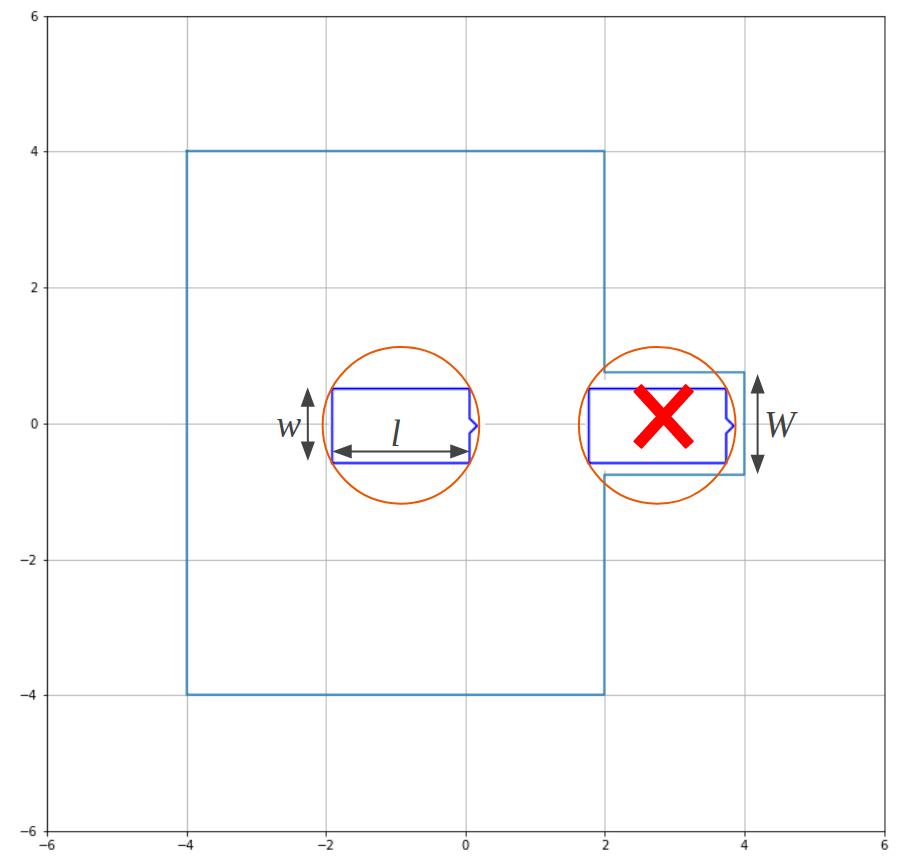
\includegraphics[scale=0.25]{images/Confined.png}
\caption{Depicting confined space given the dimensions of the robot and geometry of the environment.}
\label{Fig:confined}
\end{figure}

In Figure \ref{Fig:confined}, given the width $w$ and length $l$ of the robot and width of the corridor $W$, the area where $w < W < l$ is considered confined space.

The proposed planner generates junctions between different spaces. For example, the robot should be able to maneuver through corridors as shown in Figure \ref{Fig:maneuver}(a). The green highlighted areas are the junctions which would hold information on how the robot should enter or exit the corridor. Doorways which can be considered as shortened corridors and can also be handled similarly. Static obstacles restricting open spaces would again be treated as a narrow corridor shown in Figure \ref{Fig:maneuver}(b). 

\begin{figure}[!ht]
\centering
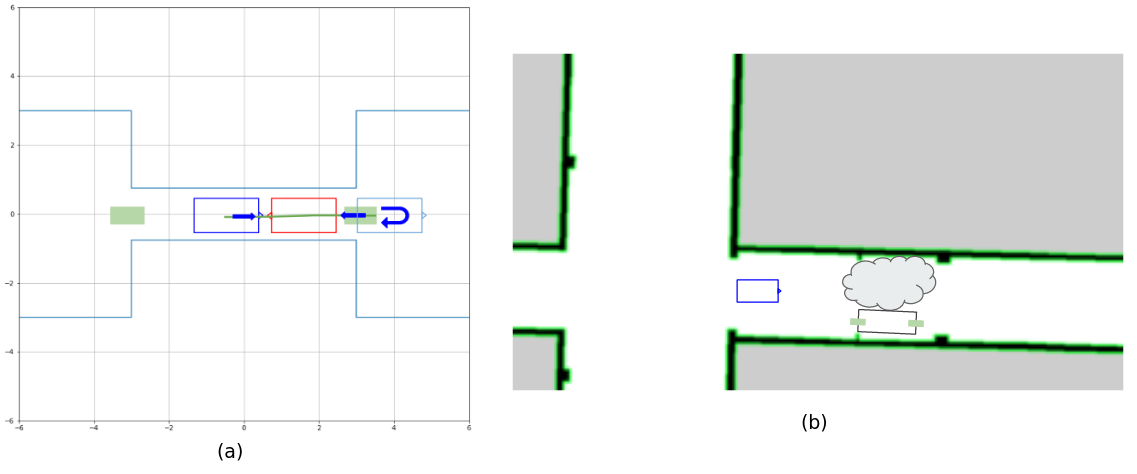
\includegraphics[scale=0.45]{images/maneuver.png}
\caption{(a) Maneuvering in corridor, given current (blue) and goal (red) poses. (b) Generating junctions for obstacle restricting open space.}
\label{Fig:maneuver}
\end{figure}

\begin{figure}[!ht]
\centering
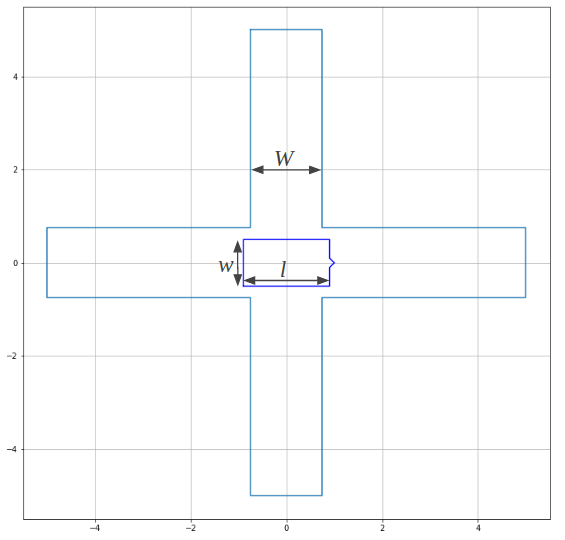
\includegraphics[scale=0.39]{images/intersection.png}
\caption{Depicting perpendicular intersection with robot dimensions.}
\label{Fig:intersect}
\end{figure}

Another use case for this planner would be to maneuver in intersections as shown in Figure \ref{Fig:intersect}. The junction generated here would be computed differently. Maneuverability is feasible only if the geometry of the robot and the intersection satisfies $w < W < l < W\sqrt{8}$. The planner would have to handle the narrow perpendicular intersections, T junctions, skewed intersections and multiple intersections for different maneuvering motions shown in Figure \ref{Fig:inter}.

\begin{figure}[!ht]
\centering
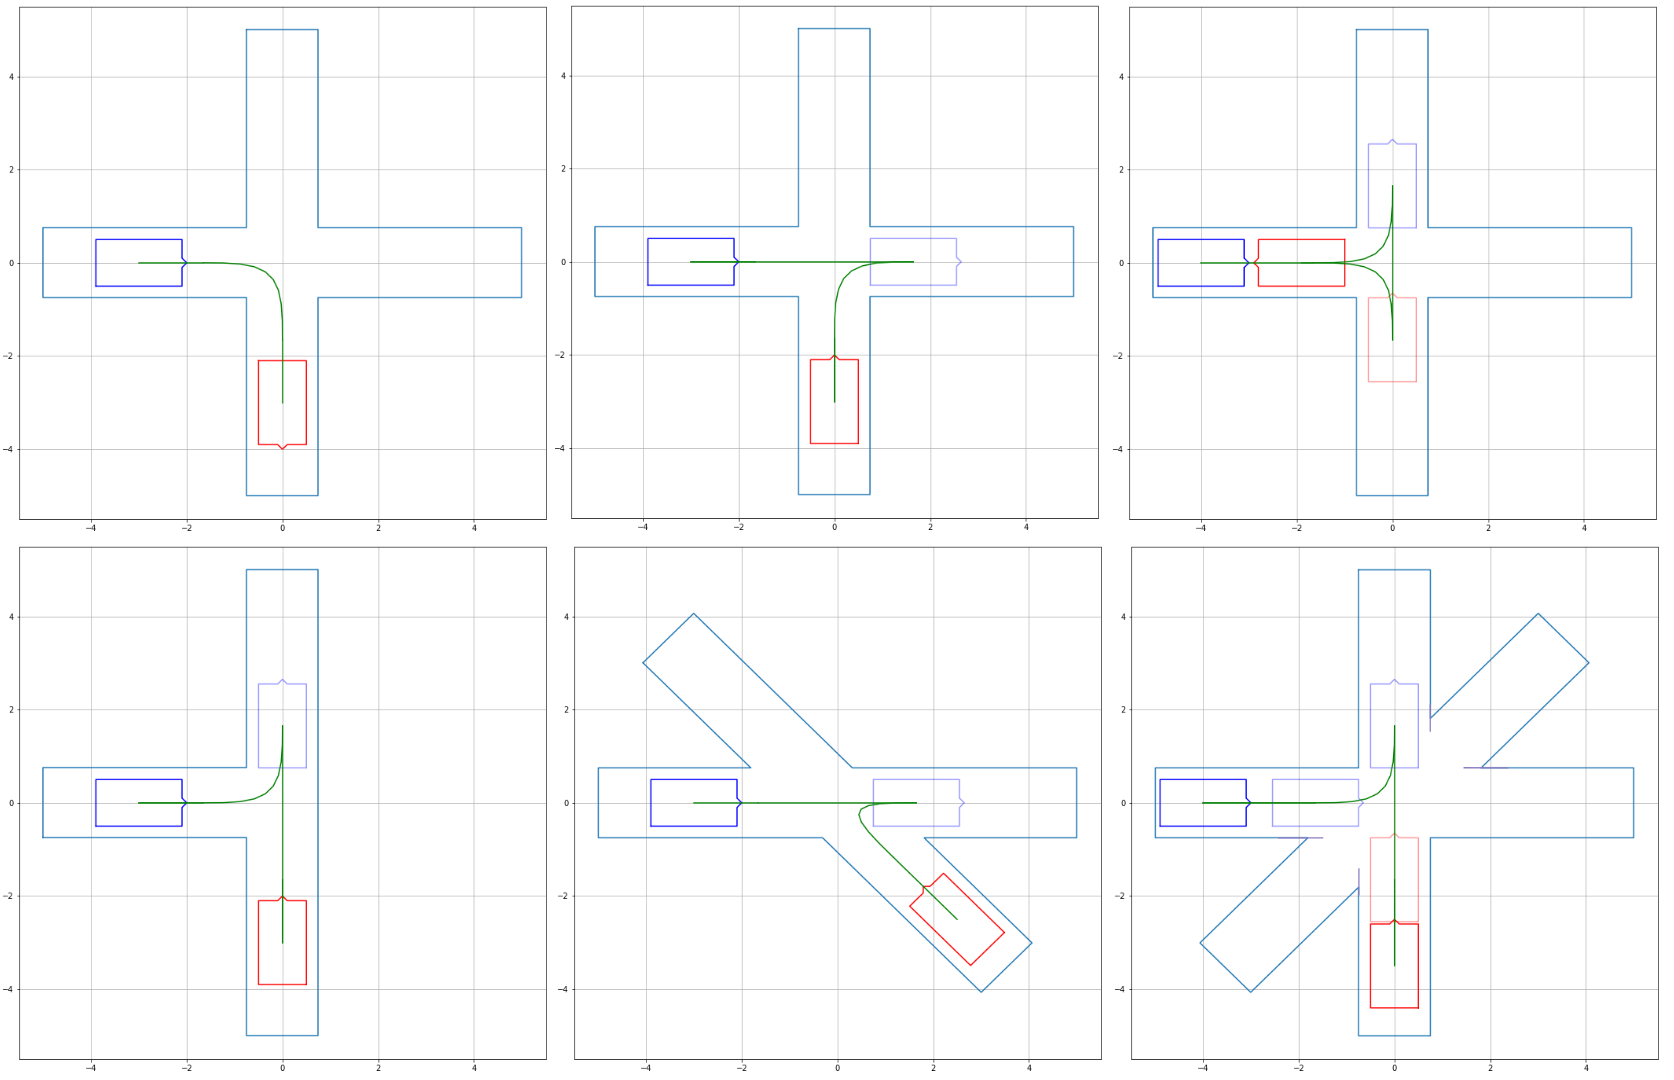
\includegraphics[scale=0.33]{images/inter.png}
\caption{Different configurations of intersections and different maneuvering motions, given current (blue) and goal (red) pose.}
\label{Fig:inter}
\end{figure}

\section{Project Plan}
\subsection{Work Packages}
\begin{enumerate}
    \item[WP1] {\bf Robot Modelling:} Setup a platform to emulate a bulky robot with a basic laser scanner in simulation and reality.
    \item[WP2] {\bf Framework:} Implement controller, localization, ROS wrapper and some common utility functions.
    \item[WP3] {\bf Setup Environments:} Build simulations with different narrow space environment configurations.   
    \item[WP4] {\bf Extend Novel Geometric Planner:} Develop an online geometric planner extended with optimization and local planning for the given model. 
    \item[WP5] {\bf Experimentation:} Conduct a set of simulations and actual experiments for different scenarios. 
    \begin{enumerate}
        \item[E1] Conduct simulation of the state of the art planners and optimizers.
        \item[E2] Conduct simulation of the novel geometric planner extended with different optimizers.
        \item[E3] The same set of experiments as in E1 and E2 will be conducted on an actual robot.
    \end{enumerate}
    \item[WP6] {\bf Project Report}
\end{enumerate}

\subsection{Milestones}
\begin{enumerate}
    \item[M1] Experimental setup for different environment and scenarios (corridor, intersections, doorways and dynamic obstacle restricting spaces).
    \item[M2] Evaluation of the state of the art planners and optimizers in simulation.
    \item[M3] Evaluation of novel geometric planner and extension with different optimizers in simulation.
    \item[M4] Evaluation of the state of the art planners and optimizers in actual robots.
    \item[M5] Evaluation of novel geometric planner and extension with different optimizers in robot.
    \item[M6] Report submission
\end{enumerate}

\subsection{Project Schedule}
\begin{figure}[!ht]
\centering
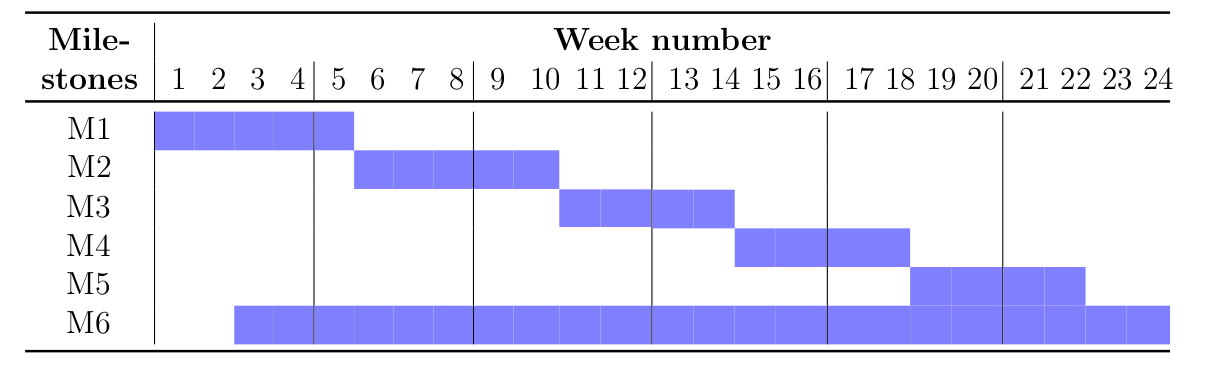
\includegraphics[scale=0.5]{images/gantt_chart.png}
\caption{Project schedule}
\label{Fig:chart}
\end{figure}

\subsection{Deliverables}
\subsubsection*{Minimum Viable}

\begin{itemize}
    \item Experimental setup for different environment and scenarios (M1)
    \item Evaluation of the state of the art planners and optimizers in simulation (M2)
    \item Demo of state of the art approaches in simulation
\end{itemize}

\subsubsection*{Expected}
\begin{itemize}
    \item Evaluation of novel geometric planner and extension with different optimizers
in simulation (M3)
    \item Evaluation of the state of the art planners and optimizers in actual robots (M4)
    \item Evaluation of novel geometric planner and extension with different optimizers
in robot (M5)
\end{itemize}

\subsubsection*{Desired}
\begin{itemize}
    \item Test in complex and dynamic (moving obstacles) environment to find where is fails
    \item Integrate into a framework which handles different spaces
\end{itemize}


\nocite{*}

\bibliographystyle{plainnat} % Use the plainnat bibliography style
\bibliography{bibliography.bib} % Use the bibliography.bib file as the source of references

\end{document}

